\section{Introduction}

Like the simple Ricardian model, it assumes an economy that produces two goods and that
can allocate its labor supply between the two sectors. Unlike the Ricardian model,
however, the specific factors model allows for the existence of factors of production
besides labor. Whereas labor is a mobile factor that can move between sectors, these
other factors are assumed to be specific. 

\subsection{Factor Proportion Theory}

The law of comparative advantage establishes the relationship between relative autarky prices and trade flows.

\begin{itemize}
    \item Countries differ in terms of factor abundance [i.e relative factor
    supply]
    \item Goods differ in terms of factor intensity [i.e relative factor demand]
\end{itemize}

Interaction between the two terms will determine differences in relative autarky prices, and in turn, the pattern of trade.


\section{Model Setup}

Let's consider an economy with two countries: $g=1,2$, and three factors of production: $L$, $K_1$, and $K_2$. 
\begin{itemize}
    \item $L$ is the mobile factor (labor) that can move between sectors.
    \item $K_1$ and $K_2$ are  ``immobile'' factors, can only be employed in one.
\end{itemize}

We denote by:
\begin{itemize}
    \item $p_1$ and $p_2$ the prices of the two goods.
    \item $w$, $r_1$ and $r_2$ the prices of the three factors.
\end{itemize}
Output of good $g$ is given by:
\begin{equation*}
    y_g = f^g(L_g, K_g)
\end{equation*}
where
\begin{itemize}
    \item $L_g$ is the amount of labor used in sector $g$.
    \item $K_g$ is the amount of capital used in sector $g$.
    \item $f^g$ is the production function of good $g$.
        \begin{itemize}
            \item Assume that $f^g$ is positive, increasing and concave in both arguments.
            \item Assume that $f^g$ is homogeneous of degree one in $(L_g, K_g)$, i.e. CRS.
        \end{itemize}
\end{itemize}
By asusming that $f^g$ is concave, we have a decreasing marginal product $f_{LL}^g < 0$ and $f_{KK} < 0$.
The model is isomorphic to DRS model(\cite{dornbusch1977comparative}): $y_g = f^g(L_g)$ with $f_{LL}^g < 0$.
Payments to specific factors under CRS is the same as profits under DRS.

The model shares the same assumpmtions as the Ricardian model below:
\begin{itemize}
    \item Perfect competition in both sectors.
    \item Full employment
    \item Endowments given, immobile across countries
    \item Constant returns to scale in each sector
\end{itemize}
Different assumpmtions are:
\begin{itemize}
    \item Labour L is mobile between sectors;
    \item Capital $K_g$ are immobile between sectors(sector specific).
\end{itemize}

\begin{figure}[htbp!]
    \centering
    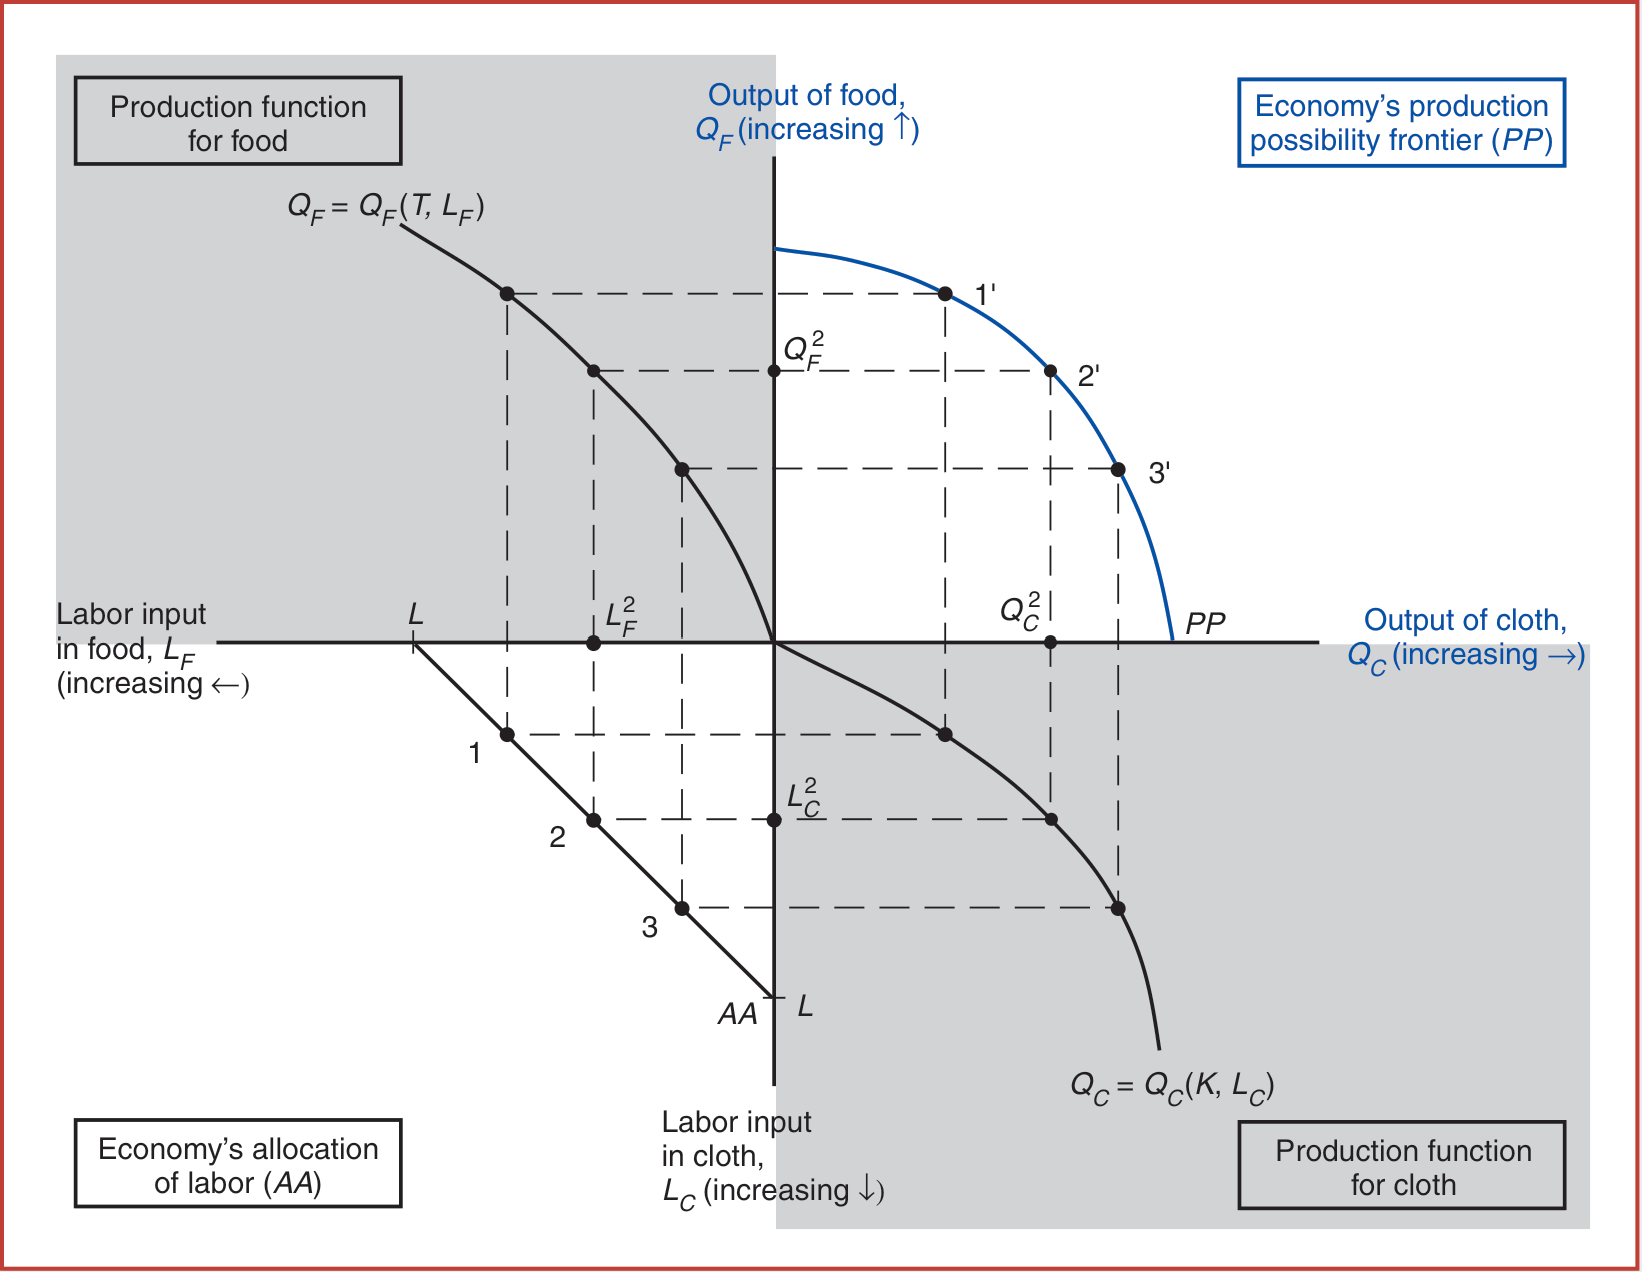
\includegraphics[width=0.8\textwidth]{figures/SFM_PPF.png}
    \caption{Production Possibility Frontier}
    \label{fig:lec4-1}
\end{figure}


Production of Good 1 and 2 is determined by the allocation of labor.
In the lower-left quadrant, the allocation between sectors can be illustrated by a point on line \textit{AA},
which represents all combinations of labor inupt of good 1 and 2 that sum up to total labor supplt $L$.

The curves in the lower-right and upper-left quadrants represent the production functions for both goods,
these allow determination of output $(Q_C^2, Q_F^2)$ given output.